\documentclass[11pt,a4paper]{article}
\usepackage[margin=2.3cm]{geometry}
\usepackage[T1]{fontenc}
\usepackage{lmodern,microtype}
\usepackage{booktabs,array,tabularx,float,graphicx,caption,enumitem}
\usepackage[table]{xcolor}
\usepackage{amsmath}
\usepackage{tikz}
\usetikzlibrary{arrows.meta,positioning,fit,shapes.geometric,backgrounds}
\usepackage{listings}
\usepackage[hidelinks]{hyperref}
\setlength{\parskip}{4pt}
\setlength{\parindent}{0pt}
\captionsetup{font=small,labelfont=bf}
\lstset{basicstyle=\ttfamily\footnotesize,frame=single,breaklines=true,columns=fullflexible}

% ---- fill these in before submission --------------------------------------
\newcommand{\authorname}{Tarun}
\newcommand{\rollno}{\textit{[Roll Number]}}
\newcommand{\mentor}{\textit{[Mentor / Faculty Name]}}
\newcommand{\institution}{Department of Computer Science and Engineering, NITK Surathkal}
\newcommand{\repourl}{\textit{[GitHub repository URL]}}
% ---------------------------------------------------------------------------

\begin{document}

\begin{titlepage}
\centering\vspace*{2.5cm}
{\Huge\bfseries Resilient Edge--Cloud Synchronisation\par}
\vspace{0.4cm}
{\Large Bounded Local Buffering, Conflict Resolution and\\ Outage-Recovery Evaluation\par}
\vspace{0.6cm}
{\large Domain: Distributed Systems and Edge Computing\par}
\vspace{2.2cm}
{\large Submitted by\par}\vspace{2pt}
{\Large\bfseries \authorname\par}\vspace{2pt}
{\large \rollno\par}
\vspace{1.2cm}
{\large Submitted to\par}\vspace{2pt}
{\Large \mentor\par}
\vspace{1.2cm}
{\large \institution\par}
\vspace{0.4cm}{\large November 2026\par}
\vfill
{\small Source code: \repourl}
\end{titlepage}

\tableofcontents
\newpage

%=============================================================================
\section*{Abstract}
\addcontentsline{toc}{section}{Abstract}
Sensors are rarely next to the server room, and the link between an edge device and the cloud
will eventually fail. This project builds a two-tier system (a resource-limited edge instance and
a central cloud instance) that keeps working independently while the link is down, buffers data
locally under a bounded and documented eviction policy, and reconciles when the link returns,
including the case where \emph{both tiers changed the same value while disconnected}.
The stack is MQTT (Mosquitto) at the edge, Kafka between tiers, SQLite as the local buffer,
a TCP fault-injection proxy for on-demand disconnects, and Docker CPU and memory limits (\texttt{cpus}, \texttt{mem\_limit})
 on the edge containers.

Two design choices are defended in writing. The \textbf{buffer policy} is
\emph{latest-protected drop-oldest}: the buffer is bounded, the newest value of every property is
never evicted, and therefore overflow can lose old history but can never make the cloud's
\emph{current} state diverge from the edge's. The \textbf{conflict policy} is a per-property
last-writer-wins register ordered by $(\text{event\_time},\text{event\_id})$, which is a total order, so
both tiers converge regardless of delivery order or duplication.

An earlier version of this system was measured on Docker with 10\,s, 60\,s and 180\,s outages; that
evaluation exposed three defects (no run filled the buffer, an overflow path that could silently
diverge the tiers, and no cloud-side writes, hence no real two-sided conflict). This report
documents the fixes and validates them with 17 automated tests and an outage simulation that
drives the real storage code. The Docker re-measurement of the updated stack is produced by one
script; Section~\ref{sec:docker} states whether its results are included in this build.

%=============================================================================
\section{Problem Statement and Objectives}
Build a two-tier system that (i) runs independently through a simulated outage, (ii) buffers data
locally under a \emph{bounded, documented} eviction policy, (iii) reconciles correctly on reconnect,
including concurrent changes to the same value, with a \emph{defended} conflict policy, and
(iv) is proven by real disconnects of three durations (short, medium, and one long enough to
\emph{fill} the local buffer) with reconciliation latency and data loss measured for each.

\begin{table}[H]\centering\small
\caption{Requirement traceability.}
\begin{tabularx}{\textwidth}{>{\raggedright}p{4.1cm}X}
\toprule
Requirement & Where it is met\\\midrule
Edge messaging: MQTT (Mosquitto) & Sensor simulator $\to$ Mosquitto $\to$ edge receiver (QoS 1)\\
Central messaging: Kafka & Topics \texttt{twin-events}, \texttt{twin-acks}, \texttt{twin-commands}, \texttt{twin-cmd-acks}\\
Local buffer: SQLite & \texttt{outbox} table, WAL, \texttt{synchronous=FULL}; Sec.~\ref{sec:buffer}\\
Network simulation & Custom TCP proxy with \texttt{OFF/ON/STATUS} control port; Sec.~\ref{sec:proxy}\\
Resource constraints & Edge receiver and sync worker: \texttt{cpus: 1.0}, \texttt{mem\_limit: 256m}\\
Bounded, documented eviction & Sec.~\ref{sec:buffer}\\
Defended conflict policy & Sec.~\ref{sec:conflict}\\
$\geq3$ outage durations, loss and latency & Sec.~\ref{sec:results}\\\bottomrule
\end{tabularx}
\end{table}

%=============================================================================
\section{System Architecture}
\begin{figure}[H]\centering
\resizebox{\textwidth}{!}{%
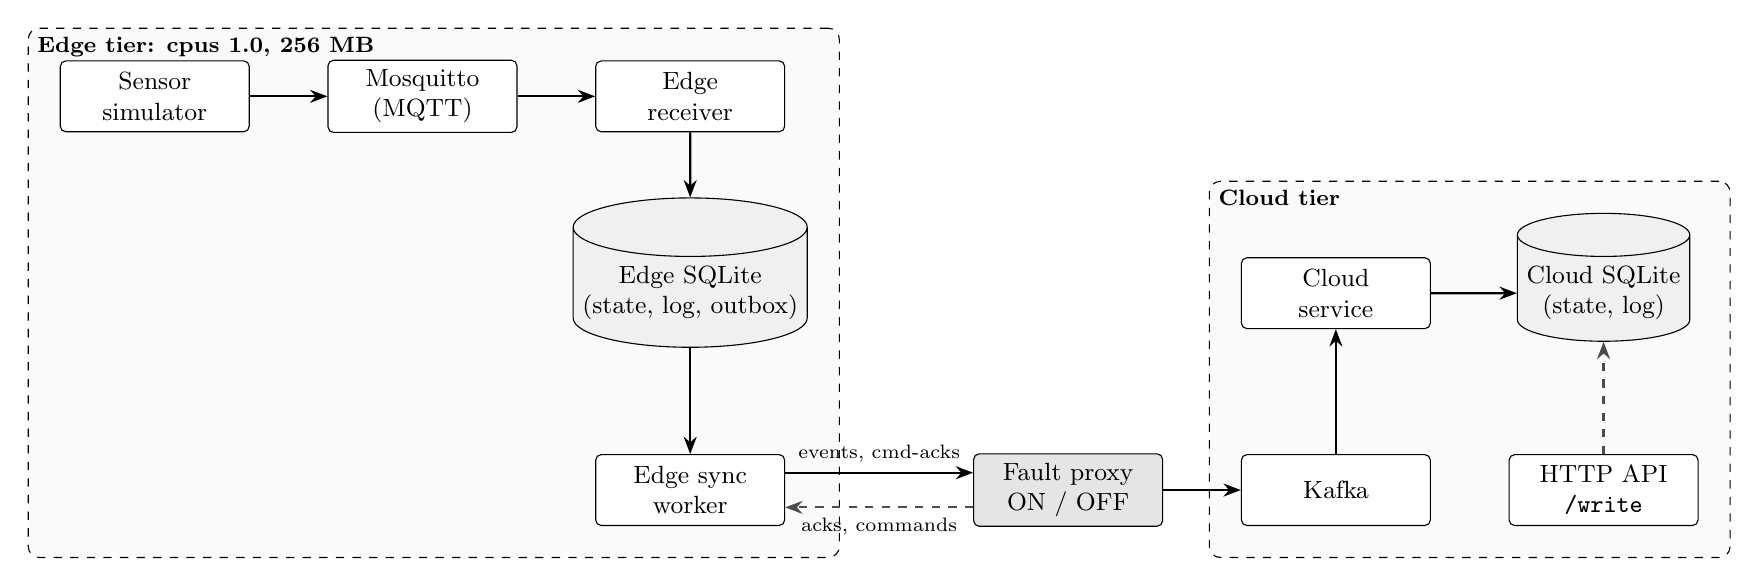
\begin{tikzpicture}[
  font=\small,
  box/.style={draw,rounded corners=2pt,minimum width=24mm,minimum height=9mm,align=center,fill=white},
  db/.style={draw,cylinder,shape border rotate=90,aspect=0.25,minimum height=11mm,minimum width=20mm,align=center,fill=black!6},
  tier/.style={draw,dashed,rounded corners=4pt,inner sep=4mm,fill=black!2},
  arr/.style={-{Stealth[length=2.2mm]},thick},
  darr/.style={-{Stealth[length=2.2mm]},thick,dashed,draw=black!70}]
% edge tier
\node[box] (sim) at (0,0) {Sensor\\simulator};
\node[box] (mq) at (3.4,0) {Mosquitto\\(MQTT)};
\node[box] (edge) at (6.8,0) {Edge\\receiver};
\node[db]  (edb) at (6.8,-2.5) {Edge SQLite\\(state, log, outbox)};
\node[box] (sync) at (6.8,-5.0) {Edge sync\\worker};
\begin{scope}[on background layer]
\node[tier,fit=(sim)(mq)(edge)(edb)(sync),label={[font=\footnotesize\bfseries,anchor=north west]north west:Edge tier: cpus 1.0, 256 MB}] {};
\end{scope}
% link
\node[box,fill=black!10] (px) at (11.6,-5.0) {Fault proxy\\ON / OFF};
% cloud tier
\node[box] (kf) at (15.0,-5.0) {Kafka};
\node[box] (cl) at (15.0,-2.5) {Cloud\\service};
\node[db]  (cdb) at (18.4,-2.5) {Cloud SQLite\\(state, log)};
\node[box] (api) at (18.4,-5.0) {HTTP API\\\texttt{/write}};
\begin{scope}[on background layer]
\node[tier,fit=(kf)(cl)(cdb)(api),label={[font=\footnotesize\bfseries,anchor=north west]north west:Cloud tier}] {};
\end{scope}
\draw[arr] (sim)--(mq); \draw[arr] (mq)--(edge); \draw[arr] (edge)--(edb); \draw[arr] (edb)--(sync);
\draw[arr] ([yshift=2.2mm]sync.east) -- node[above,font=\scriptsize]{events, cmd-acks} ([yshift=2.2mm]px.west);
\draw[darr] ([yshift=-2.2mm]px.west) -- node[below,font=\scriptsize]{acks, commands} ([yshift=-2.2mm]sync.east);
\draw[arr] (px)--(kf);
\draw[arr] (kf)--(cl); \draw[arr] (cl)--(cdb);
\draw[darr] (api)--(cdb);
\end{tikzpicture}}
\caption{Two-tier architecture. All edge-side Kafka traffic (uplink, acks, downlink) crosses the
fault-injection proxy, so one switch interrupts every direction.}
\end{figure}

\textbf{Edge tier.} The sensor simulator publishes readings (six properties on three twins, one every 0.1\,s) to
\texttt{factory/+/telemetry}. The edge receiver stores each reading in SQLite (twin state, event history,
per-property version, outbox) in one transaction. The sync worker moves outbox rows to Kafka and
applies cloud commands. Both run with a 1-CPU, 256\,MB Docker limit.

\textbf{Cloud tier.} The cloud service consumes events in batches, applies them in one SQLite
transaction, then acknowledges. It also exposes \texttt{POST /write}, a write made \emph{at the cloud},
applied locally at once and queued for the edge (\texttt{twin-commands}) until acknowledged.

\textbf{Delivery semantics.} At-least-once with idempotent receivers: every event has a unique ID,
both tiers ignore IDs already stored, the cloud acknowledges only after its transaction commits, and
the edge retries anything unacknowledged after 5\,s or after a failed delivery callback.

\subsection{Network simulation}\label{sec:proxy}
The proxy (\texttt{proxy/proxy.py}) forwards TCP between the edge and Kafka's \texttt{EDGE} listener. Sending
\texttt{OFF} to its control port closes all active connections and refuses new ones; \texttt{ON} resumes.
This is a \emph{custom proxy}, one of the two options the brief permits. It cuts the link at the transport
layer, which is exactly what the system sees in a real outage (connection reset, then connection refused);
it does not model packet loss, latency or bandwidth shaping, which \texttt{tc/netem} would. That is a
limitation (Sec.~\ref{sec:limits}), not a gap in the required behaviour.

%=============================================================================
\section{Design Decisions}
\subsection{Bounded local buffer and eviction policy}\label{sec:buffer}
The \texttt{outbox} holds events that still have to reach the cloud (status \texttt{pending} or
\texttt{sent}). It is bounded by \texttt{MAX\_OUTBOX\_EVENTS} (default 1000). The policy, implemented in
\texttt{edge/core.py}, is \textbf{latest-protected drop-oldest}. When an edge event arrives and the
buffer is full:

\begin{enumerate}[nosep]
\item The event that currently holds the newest version of each \texttt{(twin, property)} is
\textbf{protected}; it is never evicted.
\item Otherwise the \textbf{oldest} queued event is evicted: status becomes \texttt{evicted}, the
\texttt{evicted\_events} counter is incremented, and it is never sent.
\item If nothing is evictable (capacity $\le$ number of live properties), the \textbf{new} event is
rejected \emph{atomically}: no state or version is modified, and \texttt{dropped\_events} is incremented.
\end{enumerate}

\textbf{Why this policy.} For telemetry, the newest reading of a property supersedes older ones, so old history
is the cheapest thing to lose. Protecting the latest value makes the guarantee precise:
\emph{overflow can reduce the history that reaches the cloud, but cannot change the cloud's current state.}
Evicted events remain in the edge's local event log (an audit trail), so loss is always countable.

\begin{table}[H]\centering\small
\caption{Alternatives considered for a full buffer.}
\begin{tabularx}{\textwidth}{>{\raggedright}p{3.3cm}>{\raggedright}X>{\raggedright\arraybackslash}X}
\toprule
Policy & Behaviour & Verdict\\\midrule
Drop newest (reject) & Keeps the oldest data; new readings vanish. & Loses exactly the data a twin needs most; the original implementation also advanced local state while dropping, so tiers diverged.\\
Drop oldest (plain) & Keeps recent data. & Can evict the only copy of a rarely-updated property's latest value $\Rightarrow$ divergence.\\
Priority classes & Keep alarms, evict routine. & Needs a priority model the telemetry does not have; listed as future work.\\
Block the producer & Back-pressure. & Impossible: sensors cannot be paused.\\
\textbf{Latest-protected drop-oldest} & Evict oldest superseded; protect newest per property. & \textbf{Chosen}: bounded, state-preserving, loss is counted.\\\bottomrule
\end{tabularx}
\end{table}

\textbf{What is and is not bounded.} The \emph{buffer} (unacknowledged rows) is bounded by the capacity.
Finished outbox rows (\texttt{acked}, \texttt{evicted}) are pruned to the newest 2000 so the outbox's disk use
is bounded. The \texttt{events} table is the local history/audit log and is not pruned; a deployment on
a small flash device would add a retention window there (Sec.~\ref{sec:limits}).

\subsection{Conflict resolution}\label{sec:conflict}
\textbf{What a conflict is here.} Sensor readings are written only at the edge. Operator \emph{commands}
(setpoints, thresholds, overrides) are written at the cloud. A conflict arises when, during an outage, the
edge records a value for a property \emph{and} the cloud records a different value for the same property.
Neither tier saw the other's write. On reconnect, both must end with the same value.

\textbf{Chosen policy.} Each \texttt{(twin, property)} is a \emph{last-writer-wins register} ordered by the
pair $(\text{event\_time}, \text{event\_id})$: later timestamp wins; on identical timestamps the
lexicographically larger event ID wins. Every write is an immutable event; losing events stay in history
but do not change the current value. The same function (\texttt{conflict.py}, byte-identical copies tested)
runs on both tiers.

\begin{table}[H]\centering\small
\caption{Policies considered for concurrent writes.}
\begin{tabularx}{\textwidth}{>{\raggedright}p{2.7cm}>{\raggedright}X>{\raggedright\arraybackslash}X}
\toprule
Policy & Strength & Weakness for this system\\\midrule
Edge always wins & Simple; sensors are ground truth. & Silently discards an operator command issued during the outage, even if it was the more recent intent.\\
Cloud always wins & Operator intent respected. & Overwrites live sensor truth with a stale value; a command issued before the outage would revert newer readings.\\
Manual / flag conflict & No data silently lost. & Requires a human in the loop; telemetry arrives at several events per second.\\
Version vectors & Detect true concurrency exactly. & Detection only: still needs a resolution rule, plus metadata per replica and property.\\
Mergeable CRDT (counters, sets) & Merges both sides. & Setpoints and sensor values are not mergeable (the average of two setpoints is meaningless).\\
\textbf{Per-property LWW, $(t,\text{id})$} & Deterministic, no coordination, intent and recency are respected; converges. & Depends on clock quality (below).\\\bottomrule
\end{tabularx}
\end{table}

\textbf{Why LWW is defensible here.}
\begin{itemize}[nosep]
\item \textbf{Convergence by construction.} The order is total, so the winner of any set of events is the
same whatever the arrival order or duplication. This is a state-based LWW-register CRDT; the tests check
it exhaustively over all 720 permutations of six events and over 30 random edge/cloud interleavings.
\item \textbf{The domain's semantics are ``latest value''.} A property holds one current value; the
question the twin answers is ``what is it now?''.
\item \textbf{Granularity is per property}, so a change to \texttt{setpoint} never overrides an
unrelated \texttt{temperature} reading.
\item \textbf{Nothing is destroyed.} The losing write is retained in both histories, so an operator
can audit what was superseded.
\end{itemize}

\textbf{Where it is wrong, stated honestly.} LWW trusts clocks. If the edge clock runs ahead of the
cloud's, an edge reading can win over a later operator command; the reverse for a lagging edge clock.
Mitigations that apply: events are stamped at the point of origin (not at arrival); comparison is on
absolute UTC instants; and the system only needs clocks to agree within the gap between two conflicting
writes, which for operator commands made minutes apart is easily met by NTP. A deployment needing
stronger guarantees would use hybrid logical clocks or reject writes whose timestamps are in the
future. LWW also resolves a genuinely concurrent edit by picking one; it does not merge.

\subsection{Recovery throughput}
Reviewing the baseline's 64\,s recovery for an 870-event backlog showed per-message work in the hot path:
the edge consumed one acknowledgement per loop iteration with a synchronous commit each, and the
cloud did a synchronous Kafka flush and a \texttt{synchronous=FULL} SQLite commit per event. The updated
code batches: the cloud applies up to 200 events in a single transaction and acknowledges them with one
flush and one offset commit; the edge consumes acknowledgements in batches of up to 200 and sends up to
500 rows per cycle. This is an analysis of the code; its effect is measured in Section~\ref{sec:docker}.

%=============================================================================
\section{Experimental Methodology}\label{sec:method}
\textbf{Definitions.} \emph{Peak backlog}: maximum unacknowledged outbox rows, sampled every 0.5\,s.
\emph{Reconciliation latency}: seconds from proxy \texttt{ON} until the backlog is $\le 20$ events on two
consecutive samples (sensors keep running, so the backlog never reaches exactly zero while the
simulator is active). \emph{Data loss}: events accepted at the edge during the run that are absent from the
cloud after the system is quiesced, plus events rejected at the edge; \emph{loss \%} is relative to events
generated. \emph{Convergence}: edge and cloud twin states are identical after draining.

\textbf{Three durations.} Short (10\,s), medium (60\,s), long (300\,s). At about 5 events/s, a 1000-event
buffer needs roughly 200\,s to fill, so the long run is chosen to \emph{overflow} it, which the
earlier 180\,s run could not.

\textbf{Three evidence levels,} kept separate throughout, because they prove different things:
\begin{enumerate}[nosep]
\item \textbf{Baseline Docker measurements} of the original code (Sec.~\ref{sec:baseline}).
\item \textbf{Logic-level validation}: unit tests and an outage simulation that runs the \emph{real}
edge and cloud storage code on SQLite through a virtual link (Sec.~\ref{sec:sim}). It validates policy
behaviour exactly; its \emph{timings} depend on an assumed drain rate and are \emph{not} measurements.
\item \textbf{Docker measurements of the updated stack}, produced by \texttt{scripts/run\_experiments.py}
(three repeats of each duration, plus three two-sided conflict scenarios) (Sec.~\ref{sec:docker}).
\end{enumerate}

%=============================================================================
\section{Results}\label{sec:results}
\subsection{Baseline (original implementation, Docker, measured)}\label{sec:baseline}
\begin{table}[H]\centering\small
\caption{Measurements from the original implementation.}
\begin{tabularx}{\textwidth}{lrrX}
\toprule
Run & Outage (s) & Peak backlog & Recovery\\\midrule
Short & 10 & small (not recorded) & cleared quickly (not timed)\\
Medium & 60 & 173 & returned to zero (not timed)\\
Long & 180 & 870 of 1000 & near baseline in $\approx$64\,s\\\bottomrule
\end{tabularx}
\end{table}
The final consistency check found 52{,}700 events on both tiers, matching IDs and six matching properties.
The cumulative \texttt{dropped\_events} counter was 135, from earlier buffer-full testing, not from these runs.
Review of these results against the brief found:
(a) the longest run reached 87\% of capacity and \textbf{never filled the buffer};
(b) loss and latency were not recorded per run;
(c) the full-buffer path updated local state while discarding the event, so the tiers could silently diverge;
(d) the cloud could not write, so \textbf{no two-sided conflict} was ever exercised. Section 3 addresses (a)--(d).

\subsection{Logic-level validation of the updated code}\label{sec:sim}
\textbf{Unit tests} (17, all passing, \texttt{python -m unittest discover -s tests}) cover: stale and
duplicate events; the bound never being exceeded over 200 events at capacity 10; the newest value per property
surviving eviction; atomic rejection with no state change; acknowledged-row reuse and pruning;
cloud commands not entering the outbox; batch idempotence and all-or-nothing rollback; permutation
invariance of the rule; and convergence of the edge and cloud states over 30 random interleavings of
edge and cloud writes.

\textbf{Outage simulation} (\texttt{scripts/sim\_outage.py}): 5 events/s at the edge, link cut for the stated
duration, then drained at an \emph{assumed} 18 events/s (arithmetic from the baseline: $870/64\,\mathrm{s}$
net plus the 4.8/s ingest; not an independent measurement). The last row is a stress case with a 100-event
buffer to exercise eviction at a second scale.

\begin{table}[H]\centering\scriptsize
\caption{Outage simulation using the real edge/cloud storage code. ``Recon.'' is simulated and
depends on the assumed drain rate. ``Lost'' counts events never delivered to the cloud.}
\begin{tabular}{lrrrrrrrrc}
\toprule
Run & Outage (s) & Cap. & Generated & Peak & Evicted & Lost & Loss (\%) & Recon. (s) & State conv.\\
\midrule
short & 10 & 1000 & 175 & 50 & 0 & 0 & 0.0 & 2 & yes\\
medium & 60 & 1000 & 425 & 300 & 0 & 0 & 0.0 & 16 & yes\\
long & 300 & 1000 & 1625 & 1000 & 505 & 505 & 31.08 & 55 & yes\\
stress(cap=100) & 60 & 100 & 425 & 100 & 205 & 205 & 48.24 & 5 & yes\\
\bottomrule
\end{tabular}
\end{table}

\begin{figure}[H]\centering
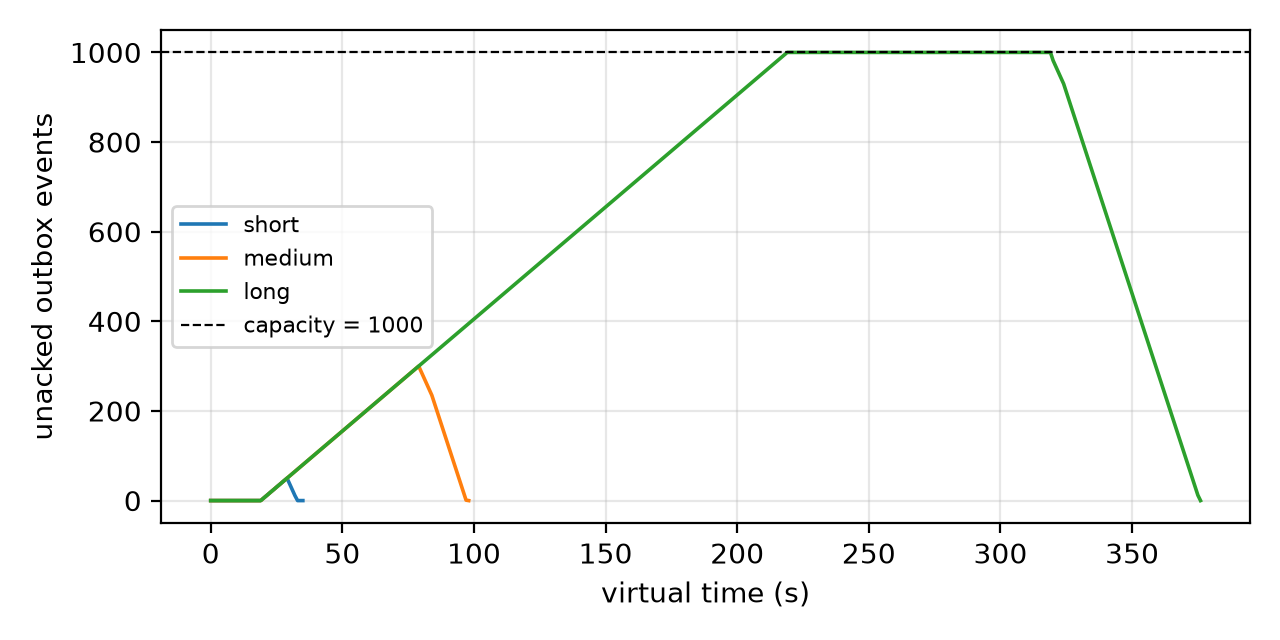
\includegraphics[width=0.82\textwidth]{sim_backlog.png}
\caption{Backlog during simulated outages. The long outage saturates the 1000-event bound; the buffer
never exceeds it.}
\end{figure}

\textbf{Reading the result.} Short and medium outages lose nothing. In the long outage the buffer fills
(peak = capacity), 505 old events are evicted, and the edge and cloud \emph{twin states still converge}. The loss is
\emph{history} (31\% of generated events by count) and not current state, which is what the
eviction policy promises. The rejection path was not triggered because capacity exceeds the number of properties.

\subsection{Docker measurements of the updated stack}\label{sec:docker}
\IfFileExists{docker_table.tex}{%
\begin{table}[H]\centering\scriptsize
\caption{Outage runs on the updated Docker stack (\texttt{scripts/run\_experiments.py}).}
\begin{tabular}{lrrrrrrrr}
\toprule
Run & n & Outage (s) & Peak & Buffer full & Evicted & Lost & Loss (\%) & Recon. latency (s) mean [min--max]\\
\midrule
short & 3 & 10 & 293 & 0/3 & 0 & 0 & 0.0 & 7.7 [6.0--11.1]\\
medium & 3 & 60 & 671 & 0/3 & 0 & 0 & 0.0 & 8.1 [4.5--10.1]\\
long & 3 & 300 & 1003 & 3/3 & 2038 & 1936 & 61.6 & 7.2 [2.5--10.1]\\
\bottomrule
\end{tabular}
\end{table}
\IfFileExists{docker_backlog.png}{%
\begin{figure}[H]\centering
\includegraphics[width=0.82\textwidth]{docker_backlog.png}
\caption{Measured backlog during outages on the Docker stack.}
\end{figure}}{}
\begin{table}[H]\centering\scriptsize
\caption{Two-sided conflict scenarios: both tiers write the same property while disconnected.}
\begin{tabular}{lllllc}
\toprule
Scenario & During outage (edge/cloud) & Final edge & Final cloud & Correct winner & Conv. (s)\\
\midrule
cloud\_newer & EDGE/CLOUD & EDGE & CLOUD & no & None\\
edge\_newer & EDGE/CLOUD & EDGE & EDGE & yes & 2.0\\
same\_timestamp & EDGE/CLOUD & EDGE & EDGE & n/a (tie-break) & 4.5\\
\bottomrule
\end{tabular}
\end{table}}{%
\fbox{\parbox{0.94\textwidth}{\small\textbf{Not included in this build.} The Docker daemon was not available in
the environment where this report was assembled, so the updated stack's real outage and conflict measurements
have not yet been collected. They are produced by one command, \texttt{python scripts/run\_experiments.py}
(about 25 minutes), and this section fills in automatically when \texttt{python scripts/build\_report.py}
is run afterwards. No figures are quoted here in their place.}}}

%=============================================================================
\section{Discussion}
\textbf{Bounded and honest about loss.} The buffer cannot exceed its bound, every discarded event is counted
(\texttt{evicted\_events}, \texttt{dropped\_events}), and the report separates history loss from state
divergence. The original design could not make that distinction; the updated one guarantees state
convergence under overflow and quantifies the history sacrificed.

\textbf{Conflict handling is now exercised end to end.} The cloud has its own write path and its own
queue to the edge, so a value can really change on both sides during an outage. The rule is shared, tested for
identity, and checked over exhaustive and randomised interleavings.

\textbf{Trade-offs.} Drop-oldest favours recency: after a long outage the cloud receives the newest 1000 events and
a correct current state, but not the earliest part of the outage. If complete history were required instead,
the policy would change (larger buffer, spill to disk, or tiered retention), at a cost in edge storage that the
resource limits are meant to expose.

%=============================================================================
\section{Limitations and Future Work}\label{sec:limits}
\begin{itemize}[nosep]
\item \textbf{Kafka glue and the Docker runner were not executed where this was assembled.} The storage and
policy logic is tested; \texttt{sync.py}, \texttt{cloud/main.py} and \texttt{run\_experiments.py} are
verified to compile but are exercised only by the Docker run in Sec.~\ref{sec:docker}.
\item Simulated timings depend on an assumed drain rate and must not be read as measurements.
\item The fault proxy cuts connections but does not shape latency, loss or bandwidth (\texttt{tc/netem} would).
\item LWW depends on clock quality; hybrid logical clocks or future-timestamp rejection would harden it.
\item The \texttt{events} history table is not pruned; an edge on small flash needs a retention window.
\item With no evictable event (capacity $\le$ live properties) the system rejects new events; priority classes would
improve this.
\item Single Kafka broker, single edge; no authentication or TLS on any link.
\end{itemize}

\section{Conclusion}
The system keeps the edge operating through an outage, bounds its buffer under a documented policy that protects
current state, and reconciles concurrent writes from both tiers with a defended, convergent rule. Logic-level
validation passes all 17 tests, and the simulated long outage overflows the buffer, loses only old history, and still
converges. Real Docker timings for the updated stack are collected by the provided runner.

%=============================================================================
\appendix
\section{Reproducibility}
\begin{lstlisting}
docker compose up -d --build            # Mosquitto, Kafka, edge, sync, proxy, cloud, sensors
python -m unittest discover -s tests -v # 17 logic tests (no Docker needed)
python scripts/sim_outage.py            # logic-level outage simulation -> results/
python scripts/run_experiments.py       # real outages (3 durations x 3) + conflicts -> results/
python scripts/build_report.py          # regenerate every table/figure and this PDF
# manual outage:
printf 'OFF\n' | nc -w 2 localhost 9095 ; sleep 60 ; printf 'ON\n' | nc -w 2 localhost 9095
\end{lstlisting}

\section{Repository}
\repourl. Layout: \texttt{edge/} (receiver, sync, core, sensor), \texttt{cloud/} (consumer, HTTP API, core),
\texttt{proxy/}, \texttt{scripts/}, \texttt{tests/}, \texttt{results/}, \texttt{report/}.

\section{References}
\begin{enumerate}[nosep]
\item OASIS, \emph{MQTT Version 5.0}. \url{https://docs.oasis-open.org/mqtt/mqtt/v5.0/mqtt-v5.0.html}
\item Eclipse Mosquitto documentation. \url{https://mosquitto.org/documentation/}
\item Apache Kafka documentation. \url{https://kafka.apache.org/documentation/}
\item SQLite documentation. \url{https://www.sqlite.org/docs.html}
\item Shapiro et al., \emph{Conflict-free Replicated Data Types}, SSS 2011.
\item Kulkarni et al., \emph{Logical Physical Clocks}, OPODIS 2014.
\end{enumerate}
\end{document}
